\scanpage{20}
\diagram{\begin{tikzcd}[ampersand replacement=\&,column sep=tiny]
D\arrow[dr,"{\text{fini}}"']\ \subset \& G_m\arrow[d,dash]\\
\&\mathbb Q
\end{tikzcd}}
\diagram{\begin{tikzcd}[ampersand replacement=\&,column sep=tiny,row sep=small]
\&\& \unsure{\bullet|0}\\
\&\& {}_n\unsure{\mathcal U|\mathcal T}\arrow[u]\arrow[d]\\
\underline{\operatorname{Hom}}(D,\arrow[d,dash] \& G_m)\arrow[d,"n"] \& {}={}\unsure{\mathcal M|\mathcal U}\arrow[d,"n"]\quad \xi\\
\underline{\operatorname{Hom}}(D, \& G_m) \& {}={}\mathcal U\arrow[d]\\
\&\& \unsure{\bullet|0}
\end{tikzcd}}

\figure{\begin{tikzpicture}[scale=.7]
\draw (0,0) .. controls (0,.6) and (.3,1.15) .. (1.08,1.58);
\end{tikzpicture}}
\[
T(\mathbb Q)\ni\xi \qquad H^1(\mathbb Q,T_\infty(\mathcal U))
\]
\figure{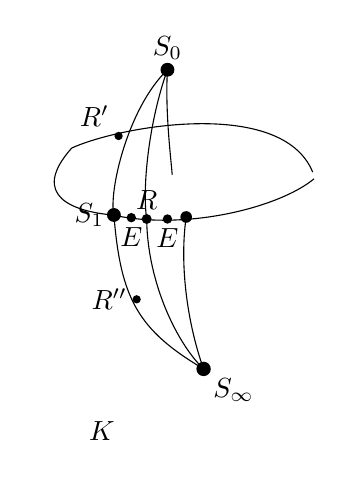
\begin{tikzpicture}[x=.85cm,y=.85cm]
\draw (3.65,.42) .. controls (3.2,1.53) and (.8,1.12) .. (.05,.78)
 .. controls (-.6,.05) and (.1,-.17) .. (.66,-.22)
 .. controls (1.75,-.46) and (3.15,-.11) .. (3.67,.32);
\draw (1.48,1.95) .. controls (.88,1.37) and (.6,.12) .. (.68,-.22)
 .. controls (.78,-1.47) and (1.04,-1.94) .. (2.02,-2.52);
\draw (1.48,1.95) .. controls (1.20,1.17) and (1.10,.18) .. (1.17,-.28)
 .. controls (1.18,-1.25) and (1.64,-2.16) .. (2.02,-2.52);
\draw (1.48,1.95) .. controls (1.44,1.28) and (1.55,.48) .. (1.55,.38);
\draw (1.76,-.25) .. controls (1.65,-1.02) and (1.8,-1.91) .. (2.02,-2.52);
\fill (1.48,1.95) circle (2.5pt) node[above] {$S_0$};
\fill (.75,.96) circle (1.5pt) node[above left] {$R'$};
\fill (.68,-.22) circle (2.5pt) node[left] {$S_1$};
\fill (.94,-.26) circle (1.7pt) node[below] {$E$};
\fill (1.17,-.28) circle (1.8pt) node[above] {$R$};
\fill (1.48,-.28) circle (1.7pt) node[below] {$E$};
\fill (1.76,-.25) circle (2.1pt);
\fill (1.02,-1.48) circle (1.5pt) node[left] {$R''$};
\fill (2.02,-2.52) circle (2.6pt) node[below right] {$S_\infty$};
\node at (.5,-3.45) {$K$};
\end{tikzpicture}}
\diagram{\begin{tikzcd}[ampersand replacement=\&,column sep=large,row sep=large]
\Gamma\arrow[r]\arrow[dr,"{\substack{\text{image de}\\\text{dim }\unsure{11|1?|n}+1?}}"'] \& \operatorname{Aff}(T_\infty(\mathcal U))\arrow[d]\\
\&\operatorname{Aut}(T_\infty(\mathcal U))
\end{tikzcd}}
Ss-groupe d'indice fini : opère \unsure{par|dans} \unsure{homothéties|hom.}

$\unsure{\xi|j}_i$ \unsure{---} \unsure{linéair\textsuperscript{t}} indép. mod \unsure{racines|premier} de 1

\diagram{\begin{tikzcd}[ampersand replacement=\&,column sep=large]
\Gamma\arrow[r]\arrow[dr]\arrow[ddr,bend right=42] \& \operatorname{Aff}(n,\widehat{\mathbb Z})\arrow[d]\quad\deleted{\text{image de}}\\
\&\widehat{\mathbb Z}^{\unsure{*|s}}\mathbin{.}\widehat{\mathbb Z}^{n}\\
\&\text{image d'indice \unsure{finie|fini} ???}
\end{tikzcd}}
% archive sheet number: 19
